\documentclass[tikz,border=3pt]{standalone}
\usetikzlibrary{arrows.meta}
\begin{document}
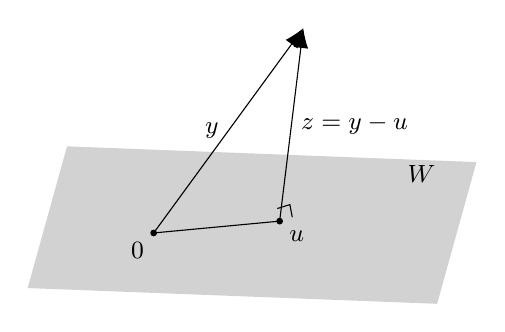
\begin{tikzpicture}[>=Latex, font=\small]
  \coordinate (O) at (0,0);
  \coordinate (U) at (1.6,0.15);
  \coordinate (P) at (1.9,2.6);

  \fill[gray!35] (-1.6,-0.7) -- (3.6,-0.9) -- (4.1,0.9) -- (-1.1,1.1) -- cycle;
  \node at (3.4,0.75) {$W$};

  \draw[-{Latex[length=2.5mm]}] (O) -- (P) node[midway, left] {$y$};
  \draw[-{Latex[length=2.5mm]}] (U) -- (P) node[midway, right] {$z=y-u$};
  \draw (O) -- (U);

  \draw (U) ++(-0.03,0.16) -- ++(0.16,0.05) -- ++(0.03,-0.16);

  \filldraw (O) circle (1pt) node[below left] {$0$};
  \filldraw (U) circle (1pt) node[below right] {$u$};
\end{tikzpicture}
\end{document}
